% Made up for the tikra benchmark.
% The DNA double helix: two backbones winding around each other, joined by base pairs.
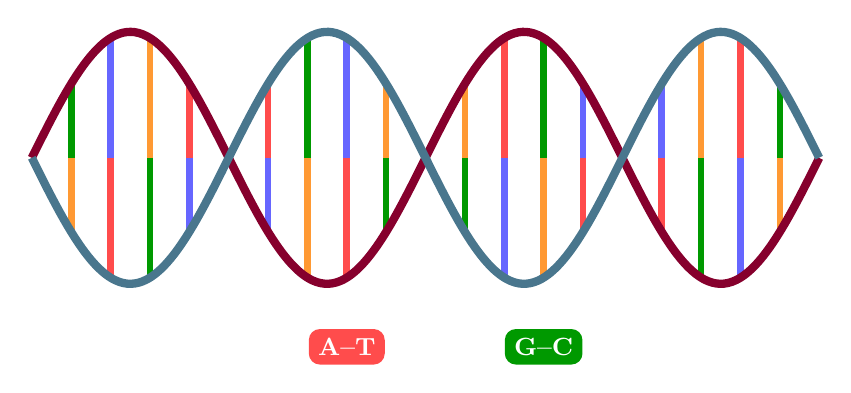
\begin{tikzpicture}[x=0.5cm, y=1cm]
  \foreach \t in {0,0.25,...,20} {
    \pgfmathsetmacro\a{1.6*sin(\t*36)}
    \pgfmathsetmacro\b{-1.6*sin(\t*36)}
    \pgfmathtruncatemacro\k{mod(round(\t*4),4)}
    \ifnum\k=0
      \pgfmathtruncatemacro\pair{mod(round(\t),4)}
      \ifcase\pair \def\cl{red!70}\def\cr{blue!60}\or \def\cl{green!60!black}\def\cr{orange!80}\or \def\cl{blue!60}\def\cr{red!70}\or \def\cl{orange!80}\def\cr{green!60!black}\fi
      \draw[line width=2.4pt, \cl] (\t,\a) -- (\t,0);
      \draw[line width=2.4pt, \cr] (\t,0) -- (\t,\b);
    \fi
  }
  \draw[line width=3pt, purple!70!black, domain=0:20, samples=200, smooth] plot (\x,{1.6*sin(\x*36)});
  \draw[line width=3pt, cyan!50!black, domain=0:20, samples=200, smooth] plot (\x,{-1.6*sin(\x*36)});
  \foreach \l/\c [count=\i] in {A--T/red!70, G--C/green!60!black} \node[fill=\c, text=white, font=\small\bfseries, rounded corners] at (3+5*\i,-2.4) {\l};
\end{tikzpicture}
